\documentclass[10pt,a4paper,oneside]{beamer}
\usepackage[utf8]{inputenc}
\usepackage[ngerman]{babel}
\usepackage{amsmath}
\usepackage{amsfonts}
\usepackage{amssymb}
\usepackage{graphicx}
\usepackage{hyperref}
\usepackage{listings}
\usepackage{enumitem}
\author{Sabine Loch\and Matthias Jakobi}
\title{Basiswissen Website (Plone)}
\usepackage{tikz}
\usepackage{environ}
\usepackage{sidecap}
\usepackage{wrapfig}

\makeatletter
\newcommand{\LogoStuRaHTW}{
    % Created by Eps2pgf 0.7.0 (build on 2008-08-24) on Fri Mar 04 12:28:07 CET 2016
\begin{pgfpicture}
\pgfpathmoveto{\pgfqpoint{-0.002cm}{-0.002cm}}
\pgfpathlineto{\pgfqpoint{30.002cm}{-0.002cm}}
\pgfpathlineto{\pgfqpoint{30.002cm}{6.213cm}}
\pgfpathlineto{\pgfqpoint{-0.002cm}{6.213cm}}
\pgfpathclose
\pgfusepath{clip}
\begin{pgfscope}
\begin{pgfscope}
\end{pgfscope}
\begin{pgfscope}
\pgfpathmoveto{\pgfqpoint{0cm}{0cm}}
\pgfpathlineto{\pgfqpoint{30cm}{0cm}}
\pgfpathlineto{\pgfqpoint{30cm}{6.211cm}}
\pgfpathlineto{\pgfqpoint{0cm}{6.211cm}}
\pgfpathclose
\pgfusepath{clip}
\definecolor{eps2pgf_color}{rgb}{0.039216,0.039216,0.082353}\pgfsetstrokecolor{eps2pgf_color}\pgfsetfillcolor{eps2pgf_color}
\pgfpathmoveto{\pgfqpoint{20.133cm}{6.211cm}}
\pgfpathlineto{\pgfqpoint{17.525cm}{1.952cm}}
\pgfpathlineto{\pgfqpoint{16.25cm}{1.952cm}}
\pgfpathlineto{\pgfqpoint{18.858cm}{6.211cm}}
\pgfpathlineto{\pgfqpoint{20.133cm}{6.211cm}}
\pgfpathclose
\pgfpathmoveto{\pgfqpoint{17.525cm}{1.952cm}}
\pgfpathlineto{\pgfqpoint{17.091cm}{1.243cm}}
\pgfpathlineto{\pgfqpoint{15.814cm}{1.243cm}}
\pgfpathlineto{\pgfqpoint{16.249cm}{1.952cm}}
\pgfpathlineto{\pgfqpoint{17.525cm}{1.952cm}}
\pgfpathclose
\pgfpathmoveto{\pgfqpoint{16.306cm}{6.211cm}}
\pgfpathlineto{\pgfqpoint{13.697cm}{1.952cm}}
\pgfpathlineto{\pgfqpoint{12.422cm}{1.952cm}}
\pgfpathlineto{\pgfqpoint{15.03cm}{6.211cm}}
\pgfpathlineto{\pgfqpoint{16.306cm}{6.211cm}}
\pgfpathclose
\pgfpathmoveto{\pgfqpoint{13.698cm}{1.952cm}}
\pgfpathlineto{\pgfqpoint{13.263cm}{1.243cm}}
\pgfpathlineto{\pgfqpoint{11.987cm}{1.243cm}}
\pgfpathlineto{\pgfqpoint{12.422cm}{1.952cm}}
\pgfpathlineto{\pgfqpoint{13.698cm}{1.952cm}}
\pgfpathclose
\pgfpathmoveto{\pgfqpoint{17.092cm}{1.243cm}}
\pgfpathlineto{\pgfqpoint{16.872cm}{0.889cm}}
\pgfpathcurveto{\pgfqpoint{16.839cm}{0.829cm}}{\pgfqpoint{16.638cm}{0.592cm}}{\pgfqpoint{16.59cm}{0.534cm}}
\pgfpathlineto{\pgfqpoint{11.623cm}{0.534cm}}
\pgfpathcurveto{\pgfqpoint{11.65cm}{0.592cm}}{\pgfqpoint{11.734cm}{0.829cm}}{\pgfqpoint{11.768cm}{0.889cm}}
\pgfpathlineto{\pgfqpoint{11.987cm}{1.243cm}}
\pgfpathlineto{\pgfqpoint{17.092cm}{1.243cm}}
\pgfpathclose
\pgfpathmoveto{\pgfqpoint{16.59cm}{0.534cm}}
\pgfpathcurveto{\pgfqpoint{16.225cm}{0.178cm}}{\pgfqpoint{15.854cm}{0cm}}{\pgfqpoint{15.481cm}{0cm}}
\pgfpathlineto{\pgfqpoint{12.078cm}{0cm}}
\pgfpathcurveto{\pgfqpoint{11.704cm}{0cm}}{\pgfqpoint{11.552cm}{0.178cm}}{\pgfqpoint{11.623cm}{0.534cm}}
\pgfpathlineto{\pgfqpoint{16.59cm}{0.534cm}}
\pgfusepath{fill}
\definecolor{eps2pgf_color}{rgb}{0.933333,0.666667,0.223529}\pgfsetstrokecolor{eps2pgf_color}\pgfsetfillcolor{eps2pgf_color}
\pgfpathmoveto{\pgfqpoint{24.988cm}{4.969cm}}
\pgfpathlineto{\pgfqpoint{24.66cm}{4.437cm}}
\pgfpathcurveto{\pgfqpoint{24.621cm}{4.377cm}}{\pgfqpoint{24.414cm}{4.141cm}}{\pgfqpoint{24.371cm}{4.083cm}}
\pgfpathlineto{\pgfqpoint{23.163cm}{4.083cm}}
\pgfpathlineto{\pgfqpoint{23.711cm}{4.969cm}}
\pgfpathlineto{\pgfqpoint{24.988cm}{4.969cm}}
\pgfpathclose
\pgfpathmoveto{\pgfqpoint{23.611cm}{2.84cm}}
\pgfpathcurveto{\pgfqpoint{23.591cm}{2.781cm}}{\pgfqpoint{23.504cm}{2.545cm}}{\pgfqpoint{23.465cm}{2.486cm}}
\pgfpathlineto{\pgfqpoint{22.272cm}{0.534cm}}
\pgfpathlineto{\pgfqpoint{20.996cm}{0.534cm}}
\pgfpathlineto{\pgfqpoint{22.354cm}{2.84cm}}
\pgfpathlineto{\pgfqpoint{23.611cm}{2.84cm}}
\pgfpathclose
\pgfpathmoveto{\pgfqpoint{23.139cm}{1.952cm}}
\pgfpathlineto{\pgfqpoint{22.812cm}{1.421cm}}
\pgfpathlineto{\pgfqpoint{21.536cm}{1.421cm}}
\pgfpathlineto{\pgfqpoint{21.863cm}{1.952cm}}
\pgfpathlineto{\pgfqpoint{23.139cm}{1.952cm}}
\pgfpathclose
\pgfpathmoveto{\pgfqpoint{22.705cm}{1.243cm}}
\pgfpathlineto{\pgfqpoint{22.379cm}{0.712cm}}
\pgfpathlineto{\pgfqpoint{21.104cm}{0.712cm}}
\pgfpathlineto{\pgfqpoint{21.429cm}{1.243cm}}
\pgfpathlineto{\pgfqpoint{22.705cm}{1.243cm}}
\pgfpathclose
\pgfpathmoveto{\pgfqpoint{22.272cm}{0.534cm}}
\pgfpathlineto{\pgfqpoint{21.944cm}{0cm}}
\pgfpathlineto{\pgfqpoint{20.667cm}{0cm}}
\pgfpathlineto{\pgfqpoint{20.996cm}{0.534cm}}
\pgfpathlineto{\pgfqpoint{22.272cm}{0.534cm}}
\pgfpathclose
\pgfpathmoveto{\pgfqpoint{25.297cm}{5.501cm}}
\pgfpathlineto{\pgfqpoint{20.211cm}{5.501cm}}
\pgfpathlineto{\pgfqpoint{20.645cm}{6.211cm}}
\pgfpathlineto{\pgfqpoint{24.897cm}{6.211cm}}
\pgfpathcurveto{\pgfqpoint{25.272cm}{6.211cm}}{\pgfqpoint{25.509cm}{6.06cm}}{\pgfqpoint{25.297cm}{5.501cm}}
\pgfpathmoveto{\pgfqpoint{25.297cm}{5.501cm}}
\pgfpathcurveto{\pgfqpoint{25.27cm}{5.441cm}}{\pgfqpoint{25.237cm}{5.383cm}}{\pgfqpoint{25.2cm}{5.325cm}}
\pgfpathlineto{\pgfqpoint{24.987cm}{4.969cm}}
\pgfpathlineto{\pgfqpoint{19.883cm}{4.969cm}}
\pgfpathlineto{\pgfqpoint{20.211cm}{5.501cm}}
\pgfpathlineto{\pgfqpoint{25.297cm}{5.501cm}}
\pgfpathclose
\pgfpathmoveto{\pgfqpoint{21.16cm}{4.969cm}}
\pgfpathlineto{\pgfqpoint{20.61cm}{4.083cm}}
\pgfpathlineto{\pgfqpoint{19.335cm}{4.083cm}}
\pgfpathlineto{\pgfqpoint{19.883cm}{4.969cm}}
\pgfpathlineto{\pgfqpoint{21.16cm}{4.969cm}}
\pgfpathclose
\pgfpathmoveto{\pgfqpoint{24.371cm}{4.083cm}}
\pgfpathcurveto{\pgfqpoint{24.005cm}{3.727cm}}{\pgfqpoint{23.638cm}{3.55cm}}{\pgfqpoint{23.27cm}{3.55cm}}
\pgfpathlineto{\pgfqpoint{19.016cm}{3.55cm}}
\pgfpathlineto{\pgfqpoint{19.335cm}{4.083cm}}
\pgfpathlineto{\pgfqpoint{24.371cm}{4.083cm}}
\pgfpathclose
\pgfpathmoveto{\pgfqpoint{23.611cm}{2.84cm}}
\pgfpathlineto{\pgfqpoint{18.575cm}{2.84cm}}
\pgfpathlineto{\pgfqpoint{19.018cm}{3.558cm}}
\pgfpathlineto{\pgfqpoint{23.22cm}{3.55cm}}
\pgfpathcurveto{\pgfqpoint{23.595cm}{3.55cm}}{\pgfqpoint{23.682cm}{3.196cm}}{\pgfqpoint{23.611cm}{2.84cm}}
\pgfpathmoveto{\pgfqpoint{20.295cm}{3.558cm}}
\pgfpathlineto{\pgfqpoint{18.445cm}{0.534cm}}
\pgfpathlineto{\pgfqpoint{17.169cm}{0.534cm}}
\pgfpathlineto{\pgfqpoint{19.018cm}{3.558cm}}
\pgfpathlineto{\pgfqpoint{20.295cm}{3.558cm}}
\pgfpathclose
\pgfpathmoveto{\pgfqpoint{19.311cm}{1.952cm}}
\pgfpathlineto{\pgfqpoint{18.985cm}{1.421cm}}
\pgfpathlineto{\pgfqpoint{17.708cm}{1.421cm}}
\pgfpathlineto{\pgfqpoint{18.035cm}{1.952cm}}
\pgfpathlineto{\pgfqpoint{19.311cm}{1.952cm}}
\pgfpathclose
\pgfpathmoveto{\pgfqpoint{18.879cm}{1.243cm}}
\pgfpathlineto{\pgfqpoint{18.549cm}{0.712cm}}
\pgfpathlineto{\pgfqpoint{17.276cm}{0.712cm}}
\pgfpathlineto{\pgfqpoint{17.601cm}{1.243cm}}
\pgfpathlineto{\pgfqpoint{18.879cm}{1.243cm}}
\pgfpathclose
\pgfpathmoveto{\pgfqpoint{18.445cm}{0.534cm}}
\pgfpathlineto{\pgfqpoint{18.118cm}{0cm}}
\pgfpathlineto{\pgfqpoint{16.842cm}{0cm}}
\pgfpathlineto{\pgfqpoint{17.169cm}{0.534cm}}
\pgfpathlineto{\pgfqpoint{18.445cm}{0.534cm}}
\pgfusepath{fill}
\definecolor{eps2pgf_color}{rgb}{0.039216,0.039216,0.082353}\pgfsetstrokecolor{eps2pgf_color}\pgfsetfillcolor{eps2pgf_color}
\pgfpathmoveto{\pgfqpoint{28.579cm}{0cm}}
\pgfpathlineto{\pgfqpoint{27.134cm}{0cm}}
\pgfpathlineto{\pgfqpoint{27.458cm}{1.421cm}}
\pgfpathlineto{\pgfqpoint{28.902cm}{1.421cm}}
\pgfpathlineto{\pgfqpoint{28.579cm}{0cm}}
\pgfpathclose
\pgfpathmoveto{\pgfqpoint{29.679cm}{4.792cm}}
\pgfpathlineto{\pgfqpoint{26.974cm}{4.792cm}}
\pgfpathlineto{\pgfqpoint{28.384cm}{6.211cm}}
\pgfpathlineto{\pgfqpoint{30cm}{6.211cm}}
\pgfpathlineto{\pgfqpoint{29.679cm}{4.792cm}}
\pgfpathclose
\pgfpathmoveto{\pgfqpoint{29.185cm}{2.662cm}}
\pgfpathlineto{\pgfqpoint{27.739cm}{2.662cm}}
\pgfpathlineto{\pgfqpoint{28.177cm}{4.552cm}}
\pgfpathlineto{\pgfqpoint{26.294cm}{2.662cm}}
\pgfpathlineto{\pgfqpoint{24.848cm}{2.662cm}}
\pgfpathlineto{\pgfqpoint{26.974cm}{4.792cm}}
\pgfpathlineto{\pgfqpoint{29.679cm}{4.792cm}}
\pgfpathlineto{\pgfqpoint{29.185cm}{2.662cm}}
\pgfpathclose
\pgfpathmoveto{\pgfqpoint{29.064cm}{2.131cm}}
\pgfpathlineto{\pgfqpoint{24.317cm}{2.131cm}}
\pgfpathlineto{\pgfqpoint{24.848cm}{2.662cm}}
\pgfpathlineto{\pgfqpoint{29.185cm}{2.662cm}}
\pgfpathlineto{\pgfqpoint{29.064cm}{2.131cm}}
\pgfpathclose
\pgfpathmoveto{\pgfqpoint{28.902cm}{1.421cm}}
\pgfpathlineto{\pgfqpoint{23.612cm}{1.421cm}}
\pgfpathlineto{\pgfqpoint{24.317cm}{2.131cm}}
\pgfpathlineto{\pgfqpoint{29.064cm}{2.131cm}}
\pgfpathlineto{\pgfqpoint{28.902cm}{1.421cm}}
\pgfpathclose
\pgfpathmoveto{\pgfqpoint{25.057cm}{1.421cm}}
\pgfpathlineto{\pgfqpoint{23.646cm}{0cm}}
\pgfpathlineto{\pgfqpoint{22.2cm}{0cm}}
\pgfpathlineto{\pgfqpoint{23.612cm}{1.421cm}}
\pgfpathlineto{\pgfqpoint{25.057cm}{1.421cm}}
\pgfusepath{fill}
\pgfpathmoveto{\pgfqpoint{6.837cm}{2.84cm}}
\pgfpathlineto{\pgfqpoint{5.864cm}{1.243cm}}
\pgfpathlineto{\pgfqpoint{4.586cm}{1.243cm}}
\pgfpathlineto{\pgfqpoint{5.562cm}{2.84cm}}
\pgfpathlineto{\pgfqpoint{6.837cm}{2.84cm}}
\pgfpathclose
\pgfpathmoveto{\pgfqpoint{8.907cm}{6.211cm}}
\pgfpathlineto{\pgfqpoint{8.579cm}{5.679cm}}
\pgfpathlineto{\pgfqpoint{3.543cm}{5.679cm}}
\pgfpathcurveto{\pgfqpoint{3.909cm}{6.033cm}}{\pgfqpoint{4.28cm}{6.211cm}}{\pgfqpoint{4.652cm}{6.211cm}}
\pgfpathlineto{\pgfqpoint{8.907cm}{6.211cm}}
\pgfpathclose
\pgfpathmoveto{\pgfqpoint{8.579cm}{5.679cm}}
\pgfpathlineto{\pgfqpoint{8.145cm}{4.969cm}}
\pgfpathlineto{\pgfqpoint{3.042cm}{4.969cm}}
\pgfpathlineto{\pgfqpoint{3.254cm}{5.325cm}}
\pgfpathcurveto{\pgfqpoint{3.292cm}{5.383cm}}{\pgfqpoint{3.492cm}{5.619cm}}{\pgfqpoint{3.543cm}{5.679cm}}
\pgfpathlineto{\pgfqpoint{8.579cm}{5.679cm}}
\pgfpathclose
\pgfpathmoveto{\pgfqpoint{4.318cm}{4.969cm}}
\pgfpathlineto{\pgfqpoint{3.771cm}{4.083cm}}
\pgfpathlineto{\pgfqpoint{2.494cm}{4.083cm}}
\pgfpathlineto{\pgfqpoint{3.042cm}{4.969cm}}
\pgfpathlineto{\pgfqpoint{4.318cm}{4.969cm}}
\pgfpathclose
\pgfpathmoveto{\pgfqpoint{7.148cm}{3.373cm}}
\pgfpathlineto{\pgfqpoint{2.129cm}{3.373cm}}
\pgfpathcurveto{\pgfqpoint{2.15cm}{3.432cm}}{\pgfqpoint{2.243cm}{3.669cm}}{\pgfqpoint{2.282cm}{3.727cm}}
\pgfpathlineto{\pgfqpoint{2.494cm}{4.083cm}}
\pgfpathlineto{\pgfqpoint{6.747cm}{4.083cm}}
\pgfpathcurveto{\pgfqpoint{7.121cm}{4.083cm}}{\pgfqpoint{7.213cm}{3.728cm}}{\pgfqpoint{7.148cm}{3.373cm}}
\pgfpathmoveto{\pgfqpoint{7.148cm}{3.373cm}}
\pgfpathcurveto{\pgfqpoint{7.126cm}{3.313cm}}{\pgfqpoint{7.096cm}{3.254cm}}{\pgfqpoint{7.057cm}{3.196cm}}
\pgfpathlineto{\pgfqpoint{6.837cm}{2.84cm}}
\pgfpathlineto{\pgfqpoint{2.584cm}{2.84cm}}
\pgfpathcurveto{\pgfqpoint{2.215cm}{2.84cm}}{\pgfqpoint{2.064cm}{3.016cm}}{\pgfqpoint{2.129cm}{3.373cm}}
\pgfpathlineto{\pgfqpoint{7.148cm}{3.373cm}}
\pgfpathclose
\pgfpathmoveto{\pgfqpoint{5.864cm}{1.243cm}}
\pgfpathlineto{\pgfqpoint{5.644cm}{0.889cm}}
\pgfpathcurveto{\pgfqpoint{5.611cm}{0.829cm}}{\pgfqpoint{5.411cm}{0.592cm}}{\pgfqpoint{5.362cm}{0.534cm}}
\pgfpathlineto{\pgfqpoint{0.327cm}{0.534cm}}
\pgfpathlineto{\pgfqpoint{0.76cm}{1.243cm}}
\pgfpathlineto{\pgfqpoint{5.864cm}{1.243cm}}
\pgfpathclose
\pgfpathmoveto{\pgfqpoint{5.362cm}{0.534cm}}
\pgfpathcurveto{\pgfqpoint{4.996cm}{0.178cm}}{\pgfqpoint{4.626cm}{0cm}}{\pgfqpoint{4.252cm}{0cm}}
\pgfpathlineto{\pgfqpoint{0cm}{0cm}}
\pgfpathlineto{\pgfqpoint{0.327cm}{0.534cm}}
\pgfpathlineto{\pgfqpoint{5.362cm}{0.534cm}}
\pgfusepath{fill}
\pgfpathmoveto{\pgfqpoint{11.929cm}{4.976cm}}
\pgfpathlineto{\pgfqpoint{9.216cm}{0.534cm}}
\pgfpathlineto{\pgfqpoint{7.941cm}{0.534cm}}
\pgfpathlineto{\pgfqpoint{10.654cm}{4.976cm}}
\pgfpathlineto{\pgfqpoint{11.929cm}{4.976cm}}
\pgfpathclose
\pgfpathmoveto{\pgfqpoint{9.216cm}{0.534cm}}
\pgfpathlineto{\pgfqpoint{8.889cm}{0cm}}
\pgfpathlineto{\pgfqpoint{7.612cm}{0cm}}
\pgfpathlineto{\pgfqpoint{7.941cm}{0.534cm}}
\pgfpathlineto{\pgfqpoint{9.216cm}{0.534cm}}
\pgfpathclose
\pgfpathmoveto{\pgfqpoint{14.519cm}{6.211cm}}
\pgfpathlineto{\pgfqpoint{14.085cm}{5.501cm}}
\pgfpathlineto{\pgfqpoint{8.982cm}{5.501cm}}
\pgfpathlineto{\pgfqpoint{9.416cm}{6.211cm}}
\pgfpathlineto{\pgfqpoint{14.519cm}{6.211cm}}
\pgfpathclose
\pgfpathmoveto{\pgfqpoint{14.086cm}{5.501cm}}
\pgfpathlineto{\pgfqpoint{13.759cm}{4.969cm}}
\pgfpathlineto{\pgfqpoint{8.655cm}{4.969cm}}
\pgfpathlineto{\pgfqpoint{8.982cm}{5.501cm}}
\pgfpathlineto{\pgfqpoint{14.086cm}{5.501cm}}
\pgfusepath{fill}
\end{pgfscope}
\end{pgfscope}
\end{pgfpicture}

}

\newlist{tip}{enumerate}{1}
\setlist[tip]{label=Tip: ,leftmargin=*}

\newlist{hinweis}{enumerate}{1}
\setlist[hinweis]{label=Hinweis: ,leftmargin=*}

\definecolor{htworange}{HTML}{F4A621}
\definecolor{sturadarkgray}{HTML}{DDDDDD}
\definecolor{sturagray}{HTML}{EEEEEE}

\setbeamercolor{frametitle}{fg=htworange}
\setbeamercolor{item}{fg=htworange}
\setbeamercolor{structure}{fg=htworange}

\setitemize{label=\usebeamerfont*{itemize item}%
      \usebeamercolor[fg]{itemize item}
        \usebeamertemplate{itemize item}}
\lstset{
    frame=tb, % draw a frame at the top and bottom of the code block
    tabsize=2, % tab space width
    showstringspaces=false, % don't mark spaces in strings
    numbers=left, % display line numbers on the left
    commentstyle=\color{green}, % comment color
    keywordstyle=\color{blue}, % keyword color
    stringstyle=\color{red} % string color
}
\hypersetup{
    colorlinks=true,
    linkcolor=blue,
    urlcolor=red,
    linktoc=all
}

\setbeamertemplate{headline}
{
    \leavevmode%
    \hbox{%
        \begin{beamercolorbox}[wd=\paperwidth,ht=1.0ex,dp=1ex]{secsubsec}%
            \vspace*{-4em}
            \raggedleft
            \hspace*{2em}%
            {
                    \scalebox{.08}{
                        \LogoStuRaHTW{}
                    }
            }
            %
            \hspace*{2em}%
        \end{beamercolorbox}%
    }%
}

\begin{document}
\maketitle
\frame{
    \frametitle{Quellen}
    \begin{itemize}
        \item Plone Nutzerhandbuch, Viet Schiele, \url{http://www.plone-nutzerhandbuch.de/}, Lizenz: Creative-Commons-Lizenz Namensnennung-Nicht-kommerziell-Weitergabe unter gleichen Bedingungen 2.0 Deutschland \url{http://creativecommons.org/licenses/by-nc-sa/2.0/de/}
    \end{itemize}
}
\frame{\frametitle{Inhaltsverzeichnis}\tableofcontents}

\section{Anmelden}
\frame{
    \frametitle{Anmeldung}
    \begin{figure}[!h]
        \centering
        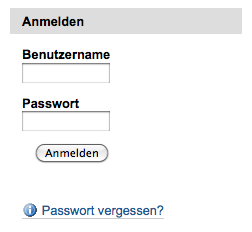
\includegraphics[width=0.66\textwidth]{../res/plone4-anmeldeportlet.png}
    \end{figure}
    \begin{description}
        \item[Benutzername] VornameNachname
        \item[Passwort] Initiales Passwort wird per E-Mail zugesendet
    \end{description}
}

\subsection{Passwort vergessen}
\frame{
    \frametitle{Passwort vergessen}
    \begin{figure}[!h]
        \centering
        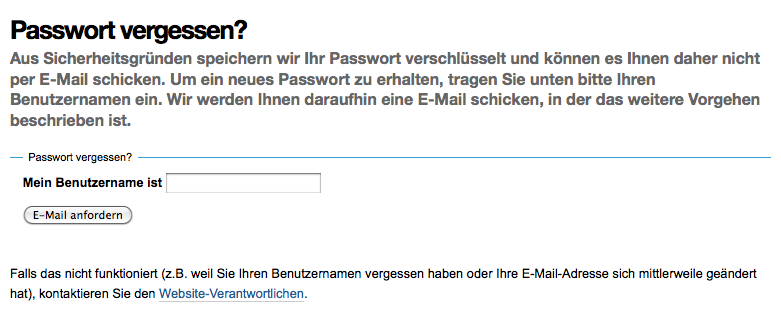
\includegraphics[width=\textwidth]{../res/plone4-passwort-zusenden.png}
    \end{figure}
    \begin{description}
        \item[Mein Benutzername ist] VornameNachname
    \end{description}
}

\section{Website Aufbau}
\frame{
    \frametitle{Website Aufbau}
    \begin{itemize}
        \item Startseite
        \item Studentinnen- \& Studentenrat
        \item weitere studentische Gremien
        \item Studentische Vertretung (an unserer Hochschule)
        \item Mitmachen
        \item Intern
        \item Hochschule
        \item Refugees Welcome
    \end{itemize}
}

\subsection{Startseite}
\frame{
    \frametitle{Website Aufbau - Startseite}
    \begin{figure}[!h]
        \centering
        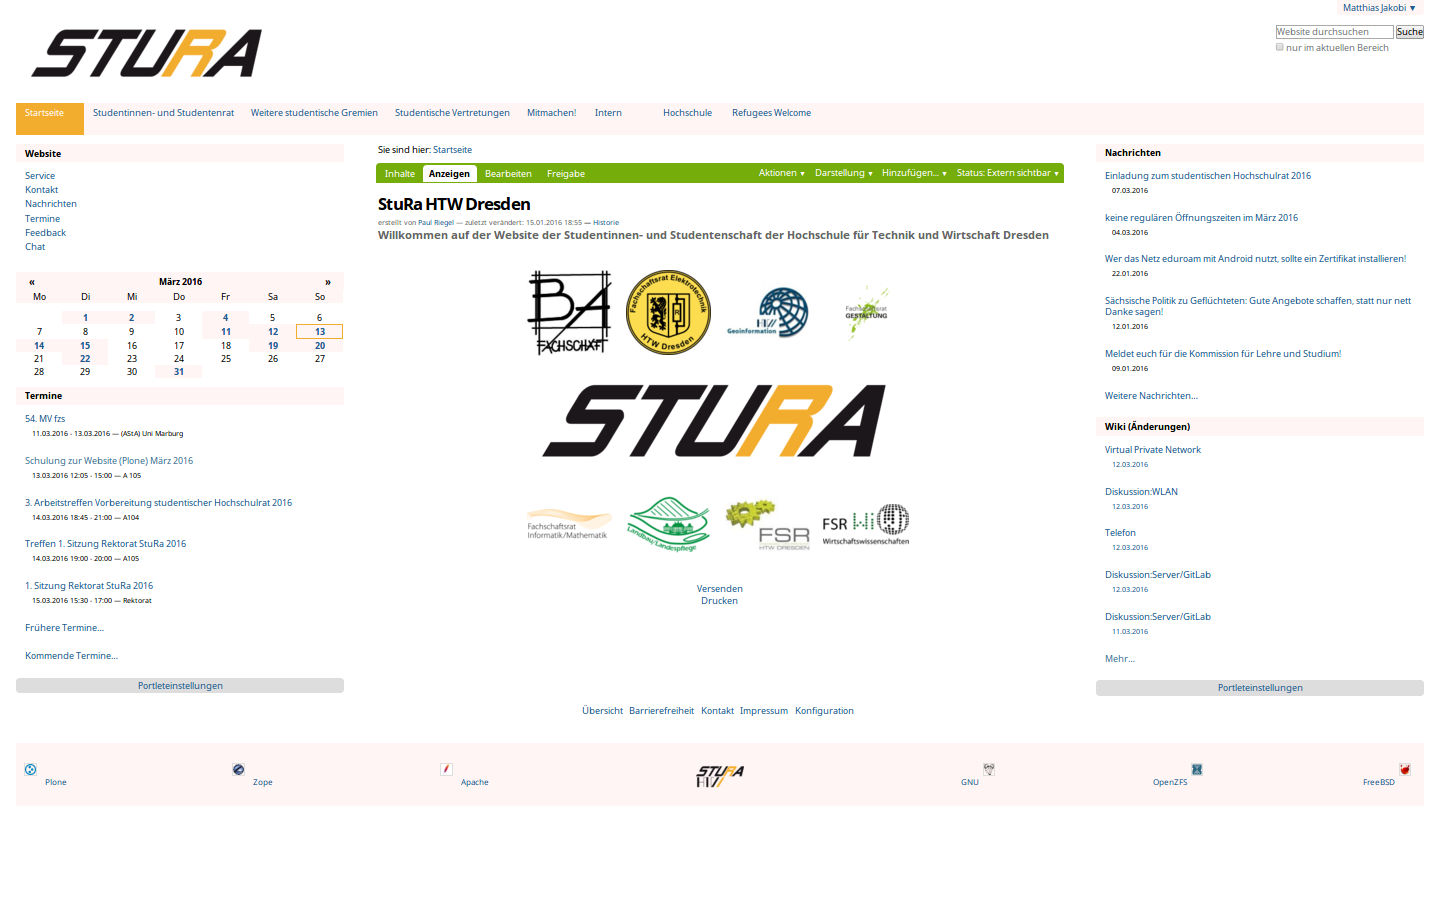
\includegraphics[width=0.9\textwidth]{../res/stura-startseite.png}
        \vspace{-20pt}
    \end{figure}
    \begin{itemize}
        \item aktuelle Inhalte
        \begin{itemize}
            \item Nachrichten
            \item Termine
            %\item Wikieinträge
        \end{itemize}
    \end{itemize}
}

\subsection{Studentinnen- \& Studentenrat}
\frame{
    \frametitle{Website Aufbau - Studentinnen- \& \newline Studentenrat}
    \begin{itemize}
        \item Übersicht, Struktur des StuRa
        \begin{itemize}
            \item Referate $\rightarrow$ Bereiche
            \item Sprecher*innen
            \item Referatskollegium
        \end{itemize}
    \end{itemize}
    \begin{itemize}
        \item allgemeines
        \begin{itemize}
            \item Sitzungen $\rightarrow$ Anträge $\rightarrow$ Protokolle
            \item Ordnungen
            \item Mitglieder
            \item Nachrichten
            \item Termine
        \end{itemize}
    \end{itemize}
}

\subsection{weitere studentische Gremien}
\frame{
    \frametitle{Website Aufbau - weitere studentische\newline Gremien}
    Ebenen: intern, lokal, regional, bundesweit, international
    \begin{itemize}
        \item Fachschaften
        \item Ausschüsse
        \item studentischer Hochschulrat
        \item Konferenz Sächsischer Studierendenschaften (KSS)
        \item freier zusammenschluss von studentinnenschaften (fzs)
        \item Studentischer Akkreditierungspool
    \end{itemize}
}

\subsection{Studentische Vertretungen}
\frame{
    \frametitle{Website Aufbau - Studentische Vertretungen}
    Ebenen: intern, lokal, regional, bundesweit, international
    \begin{itemize}
        \item Fakultätsräte
        \item Senat
        \item Erweiterter Senat
        \item Wahlausschuss HTW Dresden
        \item Verwaltungsrat Studentenwerk
        \item Unterstüzung
    \end{itemize}
}

\subsection{Mitmachen, Intern, Hochschule, Refugees Welcome}
\frame{
    \frametitle{Website Aufbau - Mitmachen, Intern,\newline Hochschule, Refugees Welcome}
    \begin{description}
        \item[Mitmachen] Übersicht der Stellausschreibungen
        \item[Intern] nur für angemeldete Nutzer*innen sichtbar;
            Daten, die nur StuRa-Mitgliedern zugänglich sein dürfen
        \item[Hochschule] Schnellverweis auf die Webseite der HTW Dresden
        \item[Refugees Welcome] Schnellverweis auf ein Antidis-Projekt
    \end{description}
}


\section{Suche}
\frame{
    \frametitle{Suche}
    \begin{description}
        \item[erneute Suche] Im Suchformular können Sie gegebenenfalls Ihre Suche ändern.
        \item[RSS-Feeds] Alternativ zu den Suchergebnissen können Sie auch Feeds abonnieren.
    %der im Kontrollfeld :doc:`konfiguration/syndizierung` angegeben wurde.
	Damit können Sie sich schnell über Änderungen in diesen Suchergebnissen informieren
    lassen.
	\item[Trefferliste]
    \end{description}
}

\subsection{Trefferliste}
\frame{
    \frametitle{Suche - Trefferliste}
    Die Suchergebnisse lassen sich noch weiter einschränken:
    \begin{itemize}
        \item nach Artikeltyp
        \item nach Datum
    \end{itemize}
    \begin{figure}[!h]
        \centering
        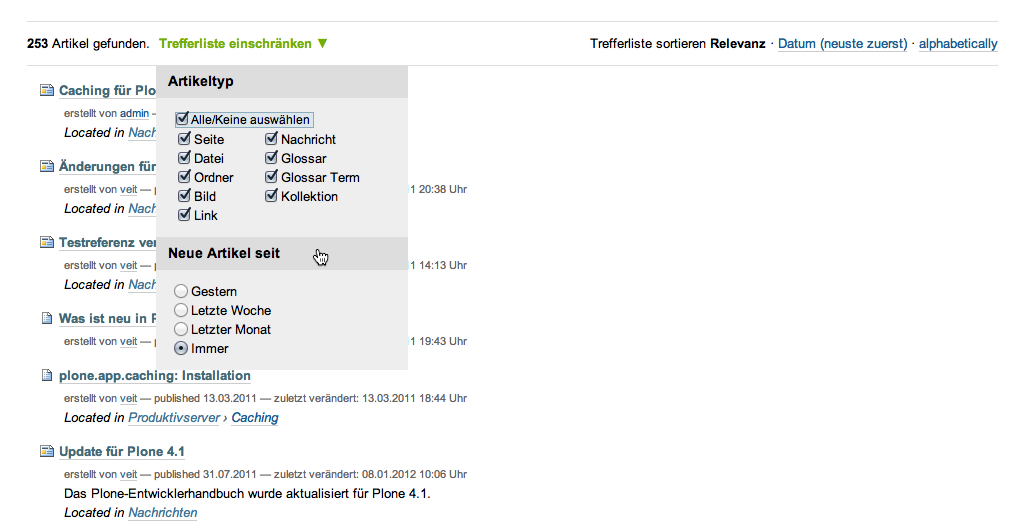
\includegraphics[width=\textwidth]{../res/suchformular.png}
    \end{figure}
}
%.. note::
%
%   Die Suche lässt sich erweitern um Suchoperatoren mit
%   :doc:`erweiterungen/textindexng/index`.


\section{Inhalte hinzufügen}
\frame{
    \frametitle{Inhalte hinzufügen}
	Artikel sind dezentral im Zuständigkeitsbereich abzulegen, d.h. im passenden Ordner des Bereiches.
	Generell ist die zentrale Ablage von z.B. Nachrichten unter ``news'' zu vermeiden. 
    Artikeltypen:
    \begin{itemize}
        \item Ordner
        \item Bild
        \item Seite
        \item Datei
        \item Link
        \item Termin
        \item Nachricht
        \item Kollektion
    \end{itemize}
}
\frame{
    \frametitle{Inhalte hinzufügen}
    \begin{figure}[!h]
        \centering
    %\begin{wrapfigure}{r}{0.4\textwidth}
        %\vspace{-20pt}
        %\begin{center}
            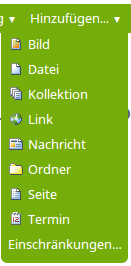
\includegraphics[width=0.33\textwidth]{../res/artikel-hinzufuegen.png}
        %\vspace{-20pt}
        %\end{center}
        \caption{Artikeltyp hinzuf\"ugen}
    %\end{wrapfigure}
    \end{figure}
}


\subsection{Kategorisierung}
\frame{
    \frametitle{Kategorisierung}
   \begin{itemize}
	\item Nicht persönliche Artikel jeden Typs sollten so umfangreich wie möglich kategorisiert werden. 
	\item Durch die Kategorisierung tauchen die Artikel in entsprechen Kollektionen auf
   \end{itemize}
   \begin{hinweis}
   \item Mehrere Stichworte müssen mit gedrückter \textit{Strg}-Taste ausgewählt werden.
   \end{hinweis}
    \begin{figure}[!h]
        \centering
        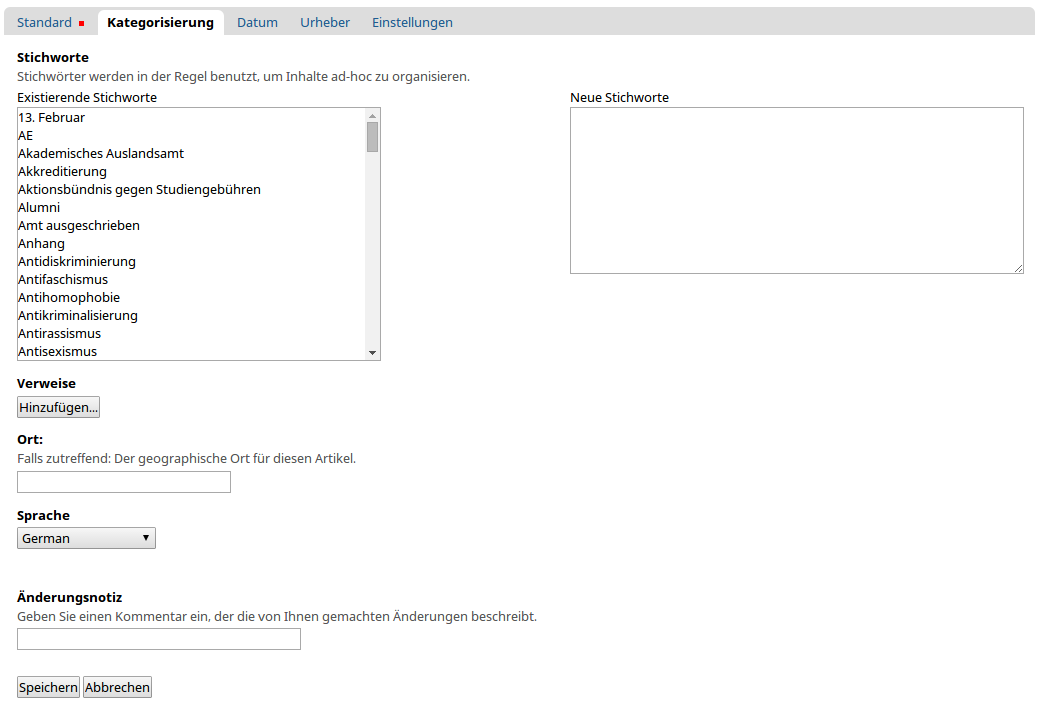
\includegraphics[width=0.66\textwidth]{../res/stura-kategorien.png}
    \end{figure}
}


\subsection{Artikeltypen}
\frame{
    \frametitle{Artikeltyp - Ordner}
    \begin{itemize}
        \item Angaben: Name, Titel, Beschreibung
        \item Startartikel: index\_html, index.html, index.htm, FrontPage
        \item Ansicht ändern
    \end{itemize}
    % Erweitertes Wissen
    %Darüberhinaus sind für Ordner noch weitere Aktionen möglich:
    %\begin{itemize}
    %    \item Syndikation
    %    \item Lokale Rollen
    %\end{itemize}
    \begin{figure}[!h]
        \centering
        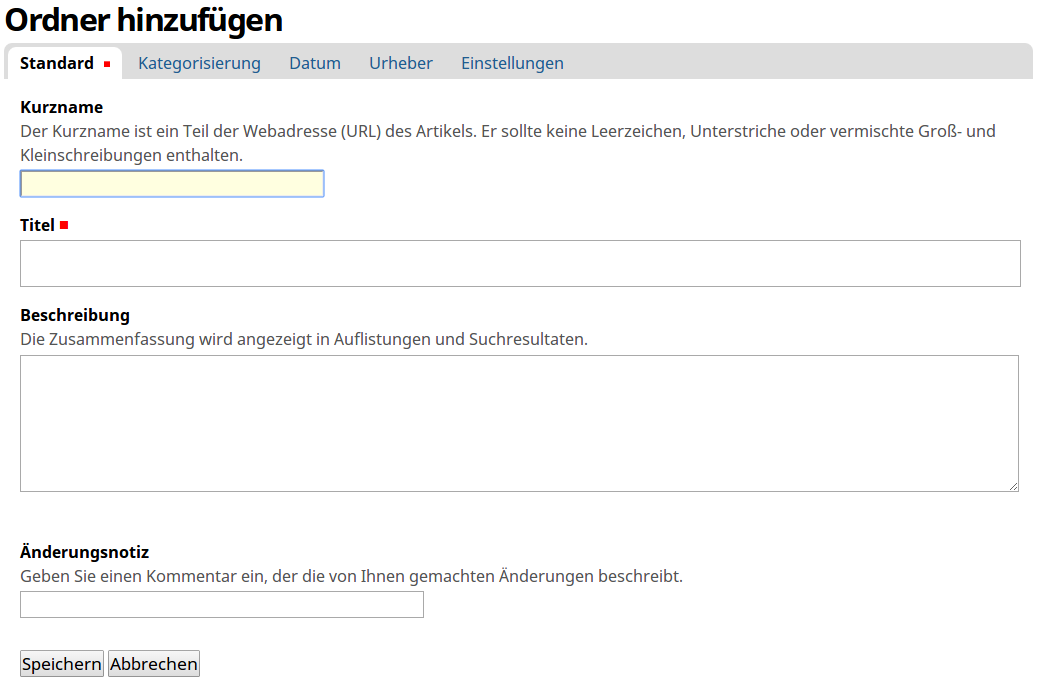
\includegraphics[width=0.75\textwidth]{../res/ordner-hinzufuegen.png}
    \end{figure}
}

\frame{
    \frametitle{Artikeltyp - Bild}
    Anschließend öffnet sich das folgende Formular:
    \begin{figure}[!h]
        \centering
        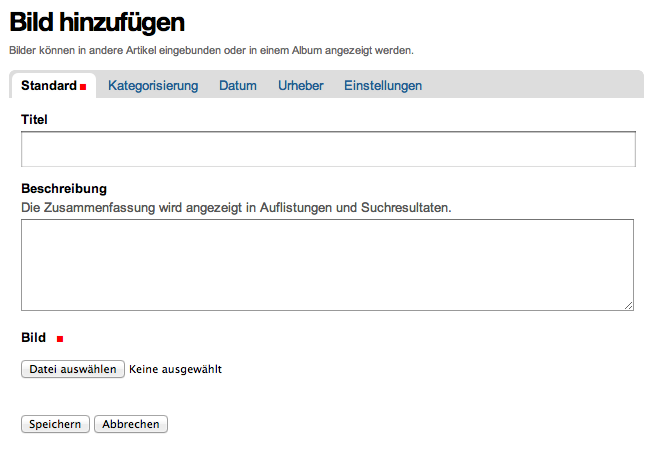
\includegraphics[width=\textwidth]{../res/bild-hinzufuegen_2.png}
    \end{figure}
}
\frame{
    \frametitle{Artikeltyp - Bild}
    \begin{description}
        \item[Titel] Aus dem Titel wird der Kurzname oder ID des Artikels gebildet.
 Wird kein Titel angegeben, behält das Bild üblicherweise seine ursprüngliche
 ID bei.

        \item[Beschreibung] Diese wird unter anderem bei der Anzeige von Suchergebnissen verwendet.

        \item[Bild] Klicken Sie auf *Datei auswählen* um auf Ihrem lokalen Computer eine Bilddatei zum Hochladen auszuwählen.
     Sie sollten die Bilder vor dem Auswählen für die Verwendung im Web
     vorbereiten. Eine kurze Anleitung hierzu finden Sie in `Bilder optimieren
     %<bilder-optimieren.html>`\_.

     Nach dem Hochladen wird Ihnen dann eine Vorschau des Bildes angezeigt.
        \item[Stichworte] Da Bilder nicht textuell erschlossen werden können, kommt den Stichworten eine besondere Bedeutung zu.
    \end{description}
}

\frame{
    \frametitle{Artikeltyp - Bild}
 \begin{tip}
     \item Eine Einführung zur Verschlagwortung von Bildern finden Sie unter
 `Verschlagwortungsstrategien
 \url{https://www.veit-schiele.de/profil/artikel/verschlagwortungsstrategien}`
 \end{tip}
}

\frame{
    \frametitle{Artikeltyp - Seite}
    \begin{itemize}
        \item Angaben: Name, Titel, Beschreibung, Eigenschaften
        \item Inhalte via Webbrowser eingebar
    \end{itemize}
    Dabei kann der Text in folgenden Formaten eingegeben werden:
    \begin{description}
        \item[HTML] ermöglicht Ihnen die direkte Eingabe von HTML;
        \item[Einfacher Text] ermöglicht Ihnen die einfache Eingabe von Text.
        \item[Markdown] ermöglicht Ihnen die direkte Eingabe mit Markdown-Syntax
    \end{description}

    Optional können Sie auch Textdateien auf den Server hochladen.
}

\frame{
    \frametitle{Artikeltyp - Datei}

	Dateiobjekte können Dateien enthalten, die heruntergeladen werden können.
	Hinzufügen:
	\begin{itemize}
	\item ``Durchsuchen\dots''-Taste klicken
	\item Verzeichnis durchsuchen, Datei auswählen
	\item ``Hochladen\dots''-Taste klicken
	\end{itemize}
	Die Bezeichnung, Beschreibung und Kategorisierung der Datei sind sehr relevant, da nur durch sie das einfache Auffinden der Datei gewährleistet werden kann.
    \begin{figure}
    %\begin{wrapfigure}{o}{\textwidth}
        %\vspace{-20pt}
        %\begin{center}
            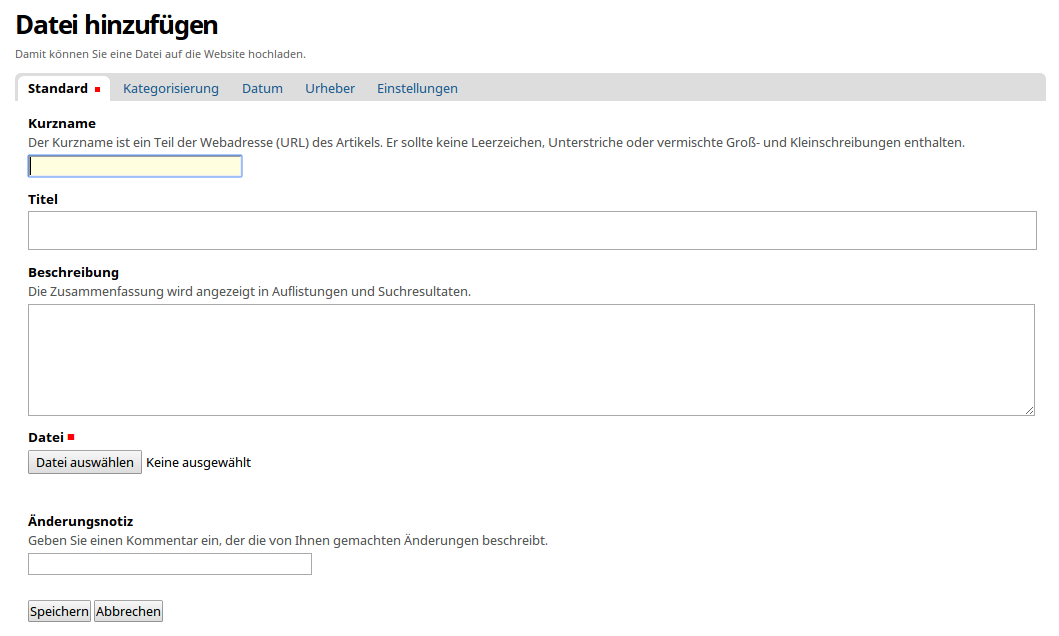
\includegraphics[width=0.5\textwidth]{../res/datei-hinzufuegen.png}
        %\vspace{-20pt}
        %\end{center}
        \caption{Datei hinzuf\"ugen}
    %\end{wrapfigure}
    \end{figure}
}

\frame{
    \frametitle{Artikeltyp - Link}
Links können als Schnellverweise gesetzt werden. 
So führt z.B. der Link \url{www.stura.htw-dresden.de/ese} für Externe direkt auf den Ordner der ESE. 
    Bitte beachten Sie bei der Angabe von externen Links die Angabe des Protokolls (z.B. ``http://'' für Webpages oder ``ftp://'' für Dateien).

    %\begin{tip}
     %   \item Auch eine Suchanfrage können Sie einfach speichern indem Sie einen Link mit der URL der Suchergebnisse erzeugen – bei jedem Aufruf des Links wird dann die Suchanfrage erneut gestartet.
    %\end{tip}

}

\frame{
    \frametitle{Artikeltyp - Termin}
    Termine sind Objekte, die im Kalender eingetragen werden. Termine sollten im Ordner \textit{Termine} der ``zuständigsten'' Stelle, z.B Referat, Bereich oder Projekt eingetragen werden. Grundsätzlich sollten Termine von der Navigation ausgeschlossen werden. Dazu ist beim Artikel über Bearbeiten und Einstellungen ein Haken bei ``Von Navigation ausschließen'' zu setzen.

    \begin{itemize}
        \item Angabe: Name, Titel, Beschreibung
        \item weiter Ereignistypen, die auch als Schlagwörter verwendet werden
    \end{itemize}
    \begin{hinweis}
        \item Wollen Sie die Einträge in dieser Liste geändert haben, wenden Sie sich bitte an die Administration der Website.
    \end{hinweis}
}

\frame{
    \frametitle{Artikeltyp - Termin}
    \begin{description}
        \item[Terminanfang] Datum und Uhrzeit des Beginns; Sie können alternativ auch im nebenstehenden Kalender den Beginn auswählen.
        \item[Terminende] Datum und Uhrzeit können alternativ auch in nebenstehendem Kalender angegeben werden.
        \item[Terminort] Hier können Sie den Ort des Termins angeben.
        \item[Terminankündigung] Ankündigungstext für den Termin; alternativ können Sie auch eine Textdatei hochladen.
        \item[Teilnehmer] Teilnehmende des Termins.
        \item[Terminart] Die Art des Termins.
        \item[URL] Hier können Sie eine Web-Adresse angeben, die weitergehende Informationen über dieses Ereignis liefert.
        \item[Kontaktname] Kontaktperson oder -organisation für das Ereignis.
        \item[Kontaktadresse] Adresse, bei der Sie weitergehende Informationen zum Ereignis erhalten können.
        \item[Kontakt-E-Mail] E-Mail-Adresse für Nachfragen.
        \item[Kontakt-Telefon] Telefonnummer für Nachfragen und Reservierungen.
    \end{description}
}

\frame{
    \frametitle{Artikeltyp - Nachricht}
    Nachrichten sind Seiten  mit Titel, optionaler Beschreibung und Bild.

    Für Nachrichten lassen sich im Gegensatz zu Seiten noch je ein Bild mit Bildtitel angeben.
    \begin{figure}[!h]
        \centering
        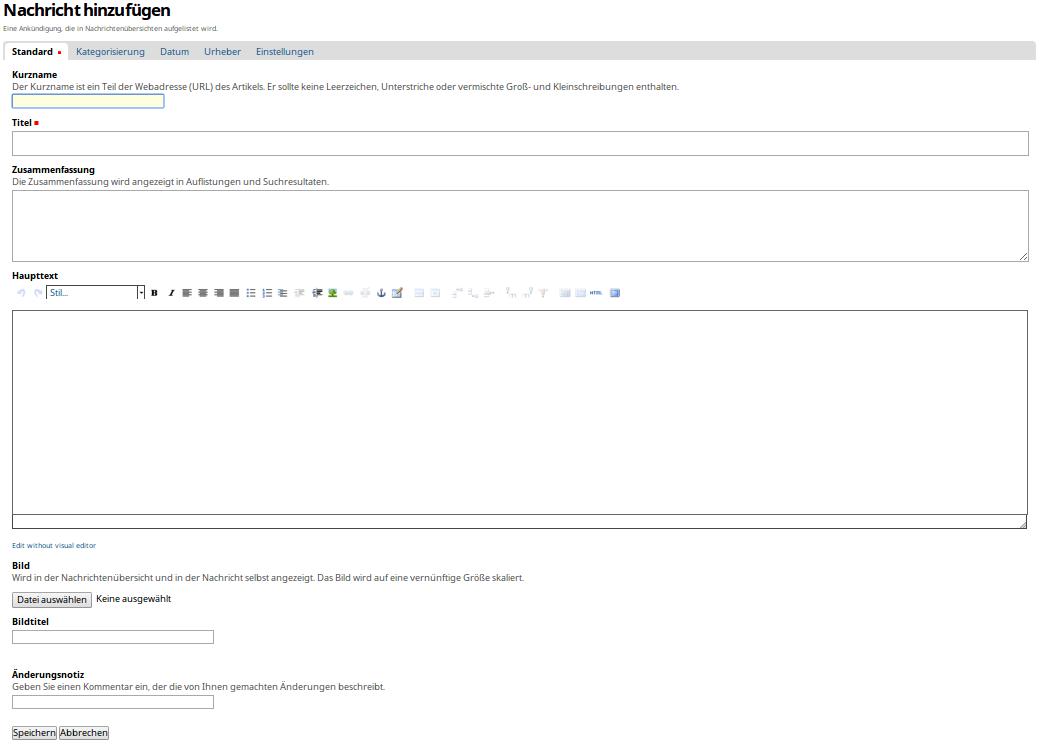
\includegraphics[width=0.75\textwidth]{../res/nachricht-hinzufuegen.png}
    \end{figure}
}

\frame{
    \frametitle{Artikeltyp - Kollektion}
    Kollektionen sind vorgefertigte Suchanfragen, die auch die Erschließung großer Datenbestände erlauben.

Kollektionen können üblicherweise nicht von allen Mitgliedern eines Portals hinzugefügt werden, sondern nur von denjenigen, die die Rollen *Website-Administrator* oder *Verwalter* innehaben. siehe: \url{www.stura.htw-dresden.de/stura/ref/verwaltung}
}

%\frame{
%    \frametitle{Artikeltyp - Kollektion}
%    \begin{figure}[!h]
%        \centering
%        \includegraphics[width=0.66\textwidth]{../res/kollektion-hinzufuegen.png}
%    \end{figure}
%   Hinzufügen-Menü mit ausgewählter Kollektion
%}
%
%\frame{
%    \frametitle{Artikeltyp - Kollektion}
%Anschließend erhalten Sie folgendes Formular:
%
%    \begin{figure}[!h]
%        \centering
%        \includegraphics[height=0.66\textheight]{../res/kollektion-hinzufuegen_2.png}
%    \end{figure}
%   Formular Kollektion hinzufügen
%
%   Unter Titel und Beschreibung sind die Felder für die Suche, deren Sortierung
%   und die Vorschau angegeben. 
%}
%
%\subsection{Artikeltyp - Kollektion - Suchbegriffe}
%\frame{
%    \frametitle{Artikeltyp - Kollektion - Suchbegriffe}
%
%Definieren Sie hier die Suchbegriffe für die Liste von Artikeln, die Sie
%angezeigt bekommen wollen. 
%
%Diese Liste wird automatisch aktualisiert. 
%
%Folgende Suchabfragen sind möglich:
%    \begin{itemize}
%        \item \dots nach Datum
%        \item \dots nach Text
%        \item \dots nach Metainformation
%    \end{itemize}
%
%}
%
%\frame{
%    \frametitle{Suchbegriffe \dots nach Datum}
%
%    \begin{figure}[!h]
%        \centering
%        \includegraphics[width=0.66\textwidth]{../res/suchbegriff-auswaehlen-datum.png}
%    \end{figure}
%   Auswählen eines Datums als Suchbegriff
%
%    Folgende Auswahlmöglichkeiten werden angeboten:
%
%    \begin{itemize}
%        \item Heute
%        \item Innerhalb der letzten ``X'' Tage
%        \item Vor dem Tag ``MM/DD/YYYY''
%        \item Nach dem Tag ``MM/DD/YYYY''
%        \item Innerhalb der nächsten ``X'' Tage
%        \item Vor dem heutigen Datum
%        \item Zwischen dem ``MM/DD/YYYY'' und ``MM/DD/YYYY''
%        \item Nach dem heutigen Datum
%    \end{itemize}
%}
%
%\frame{
%    \frametitle{Suchbegriffe \dots nach Datum}
%
%    Die Datumsangaben kann für eines der folgenden Felder angegeben werden:
%
%    \begin{description}
%        \item[Enddatum] Das Datum, ab dem der Termin nicht mehr öffentlich ist.
%        \item[Terminende] Das Datum, zu dem ein Termin endet
%        \item[Startdatum] Das Datum, zu dem ein Artikel veröffentlicht wird
%        \item[Terminanfang] Das Datum, zu dem ein Termin beginnt
%        \item[Erstellungsdatum] Das Datum, zu dem ein Artikel erstellt wurde
%        \item[Änderungsdatum] Das Datum, zu dem ein Artikel geändert wurde
%    \end{description}
%
%}
%
%\frame{
%    \frametitle{Suchbegriffe \dots nach Text}
%
%    \begin{figure}[!h]
%        \centering
%        \includegraphics[width=\textwidth]{../res/suchbegriff-auswaehlen-text.png}
%    \end{figure}
%   Auswählen von Text als Suchbegriff
%
%Je nach Feldern, in dem gesucht werden soll, wird eine Zeichenkette angegeben
%oder aus einer Liste ausgewählt 
%    \begin{description}
%        \item[Beschreibung] Die Zeichenfolge, die in der Beschreibung von Artikeln enthalten sein sollen
%        \item[Titel] Die Zeichenfolge, die im Titeln von Artikeln enthalten sein sollen
%        \item[Durchsuchter Text] Die Zeichenfolge, die in denjenigen Feldern, die auch von der allgemeinen Suche erfasst werden, vorkommt
%        \item[Stichwort] Auswahl aus der Liste aller Stichworte
%    \end{description}
%
%}
%
%\frame{
%    \frametitle{Suchbegriffe \dots nach Metainformationen}
%
%    \begin{figure}[!h]
%        \centering
%        \includegraphics[width=\textwidth]{../res/suchbegriff-auswaehlen-metaangabe.png}
%    \end{figure}
%   Auswählen der Metainformation Artikeltyp als Suchbegriff
%}
%
%\frame{
%    \frametitle{Suchbegriffe \dots nach Metainformationen}
%    Je nach den Metainformationen, in denen gesucht werden soll, können
%    unterschiedliche Angaben gemacht werden:
%
%    \begin{description}
%        \item[Artikeltyp] Aus einer Liste der Artikeltypen können ein oder mehrere Artikeltypen ausgewählt werden
%        \item[Kurzname oder ID] Die exakte ID muss angegeben werden
%        \item[Ersteller] Zwischen dem aktuellen Nutzer oder der exakten Angabe der Nutzer-ID kann ausgewählt werden
%        \item[Ort] Entweder kann ein relativer oder ein absoluter Pfad angegeben werden
%        \item[Status] Aus einer Liste aller Stadien können die gesuchten ausgewählt werden
%    \end{description}
%
%}
%
%\subsection{Artikeltyp - Kollektion - weitere Felder}
%\frame{
%    \frametitle{Artikeltyp - Kollektion - Sortierung}
%
%Die Sortierung kann nach einem der folgenden Kriterien erfolgen:
%
%\begin{description}
%    \item[Sortierbarer Titel] sortiert die Artikel in der alphabetischen Reihenfolge der Titel
%    \item[Terminende] sortiert Termine nach ihrem Enddatum
%    \item[Freigabedatum] sortiert die Artikel nach dem Datum ihrer Freigabe
%    \item[Erstellungsdatum] sortiert die Artikel nach ihrem Erstellungsdatum
%    \item[Enddatum] sortiert die Artikel nach dem Datum, zu dem sie nicht mehr freigegeben sind
%    \item[Änderungsdatum] sortiert die Artikel nach dem Datum der letzten Änderung
%    \item[Kurzname oder ID] sortiert die Artikel in alphabeitscher Reihenfolge des Kurznamens
%    \item[Terminanfang] sortiert Termine nach ihrem Startdatum
%    \item[Ersteller]
% sortiert Artikel in alphabetischer Reihenfolge der Ersteller
%    \item[Status] sortiert Artikel nach ihrem Veröffentlichungsstatus
%    \item[Stichwort] sortiert Artikel nach Stichworten
%\end{description}
%
%Die Reihenfolge der Sortierung kann jeweils umgekehrt werden.
%}
%
%\frame{
%    \frametitle{Artikeltyp - Kollektion - weitere Felder}
%    \begin{description}
%        \item[Vorschau] Zeigt eine Vorschau der ersten zehn Artikel
%        \item[Suchresultate eingrenzen] Gibt die maximale Anzahl der Suchergebnisse an.Der Standardwert ist ``1000''.
%    \end{description}
%}
%
%\frame{
%    \frametitle{Artikeltyp - Kollektion - Tabellenspalten}
%Wählen Sie, welche Felder gezeigt werden sollen, wenn im *Darstellung*-Menü *Tabelle* ausgewählt ist. 
%}
%
%\frame{
%    \frametitle{Artikeltyp - Kollektion - Tabellenspalten}
%Folgende Felder können als Tabellenspalten ausgewählt werden:
%
%    \begin{itemize}
%        \item Titel
%        \item Erstellungsdatum
%        \item Ersteller
%        \item Beschreibung
%        \item Sperrfrist
%        \item Enddatum
%        \item Löschdatum
%        \item Kurzname
%        \item Größe
%        \item Stelle
%        \item Änderungsdatum
%        \item Status
%        \item Anfangsdatum
%        \item Stichwörter
%        \item Artikeltyp
%    \end{itemize}
%
%Auch die Reihenfolge der Spalten kann angegeben werden, da neu hinzugefügte 
%Felder immer als rechte Spalte angefügt werden.
%}

\section{Veröffentlichung von Inhalten}
\frame{
 \frametitle{Veröffentlichung von Inhalten}
 Nicht jede*r Plonenutzer*in darf veröffentlichen 
 Für diese User übernimmt Referat ÖA die externe Veröffentlichung
 \subsection{Workflow}
 \begin{itemize}
 \item Referat xy erstellt Termin/Beitrag nach den inhaltlichen Regeln des StuRa
 \item Der Termin/Beitrag wird zur Veröffentlichung eingereicht
 \item Referat ÖA prüft Termin/Beitrag und nimmt bei Bedarf kleinere redaktionelle Änderungen und Korrekturen vor.
(Bei groben Fehlern wird der Termin/Beitrag zurückgewiesen)
\item Referat ÖA überprüft Kategorisierung und Relevanz für zusätzliche Veröffentlichung auf den Social       Media Sites.
\item Referat ÖA veröffentlicht den Termin/Beitrag extern.
\item Referat xy ist für die Verfolgung seiner Termine/Beiträge eigenverantwortlich.
\end{itemize}
}
\frame{
	\frametitle{Veröffentlichung von Inhalten}
    \begin{figure}[!h]
        \centering
        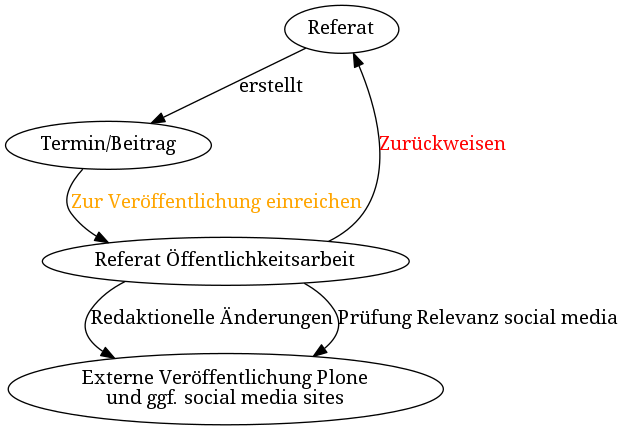
\includegraphics[height=0.8\textheight]{../res/veroeffentlichung.png}
    \end{figure}
}


\subsection{Inhalt}
\frame{
 \frametitle{Inhalt}
 Was muss vermieden werden:
 \begin{itemize}
 \item Generisches Maskulinum
 \item Fehler jeder Art
 \item Falsche Daten oder Ortsbezeichnungen
 \item Bilder ohne notwendige Rechte
 \item Falsche Verwendung von Logos
 \item Falsche oder fehlende Kategorisierung
 \item Satzzeichen, die in Rudeln auftreten 
 \end{itemize}
}

\section{Mein Ordner einrichten}
\frame{
	\frametitle{Mein Ordner einrichten}
	\begin{itemize}
		\item Mein Menue $\rightarrow$ Mein Ordner
		\item Seite hinzufügen
		\item Inhalte erstellen:
		\begin{itemize}
			\item strukturiert (mit Überschriften)
			\item Vorstellung
			\item Bild (muss kein Selfie sein)
			\item e-Mail Adresse im StuRa (mit Hyperlink)
			\item sonstiges
		\end{itemize}
		\item zur Veröffentlichung einreichen
	\end{itemize}
    Beispiele wie deine Seite aussehen kann findest du unter
    \url{https://www.stura.htw-dresden.de/members}.
}


\end{document}
